%* 
%* ------------------------------------------------------------------
%* Model Railroad System by Deepwoods Software
%* ------------------------------------------------------------------
%* SettingUp.tex - Setup
%* Created by Robert Heller on Tue Mar  5 08:39:02 2002
%* ------------------------------------------------------------------
%* Modification History: $Log$
%* Modification History: Revision 1.1  2002/11/09 21:21:07  heller
%* Modification History: Time Table User Manual
%* Modification History:
%* ------------------------------------------------------------------
%* Contents:
%* ------------------------------------------------------------------
%*  
%*     Model RR System, Version 2
%*     Copyright (C) 1994-2002  Robert Heller D/B/A Deepwoods Software
%* 			51 Locke Hill Road
%* 			Wendell, MA 01379-9728
%* 
%*     This program is free software; you can redistribute it and/or modify
%*     it under the terms of the GNU General Public License as published by
%*     the Free Software Foundation; either version 2 of the License, or
%*     (at your option) any later version.
%* 
%*     This program is distributed in the hope that it will be useful,
%*     but WITHOUT ANY WARRANTY; without even the implied warranty of
%*     MERCHANTABILITY or FITNESS FOR A PARTICULAR PURPOSE.  See the
%*     GNU General Public License for more details.
%* 
%*     You should have received a copy of the GNU General Public License
%*     along with this program; if not, write to the Free Software
%*     Foundation, Inc., 675 Mass Ave, Cambridge, MA 02139, USA.
%* 
%*  
%* 

\chapter{Setting Up}
\label{chapt:SettingUp}

When you first start up the program, it will pop up a set of dialog
boxes where it will collect some information about your layout.  This
information includes: the time frame information of your
sessions\footnote{In fast clock or ``scale'' time.}, your cab names and
color codes, your stations and the distances\footnote{In ``scale'' miles
or kilometers.}, your duplicate trackage\footnote{Typical with some
``out and back'' layouts.}, and your storage tracks.  This information
is used to create your basic train scheduling chart.  You can suppress these
pop-ups by specifying options or parameters on the command like.  See
Appendix~\ref{chapt:CLI} for more information.

\section{Saved Chart file}

The first thing you will be asked about is if you would like to load an
existing chart file.  Selecting {\tt Yes} will pop up a file selection
dialog asking for the chart file to load.  If a chart file is loaded,
the rest of the setup procedure is skipped.

\section{Session Time Frame}

If you did not load a chart file, the next thing you will be asked for
is the session time frame.  The ``Get Time Information'' dialog box
will be displayed, as shown in Figure~\ref{fig:getTimeDialog}.  The
default is 24 scale (fast clock) hours with 15 scale minute increments.
This is the horizontal dimension of the chart.  The time will be
displayed along the top in hours labeling fat vertical lines, with
thiner vertical lines at the increment value increments.

\begin{figure}
\begin{centering}
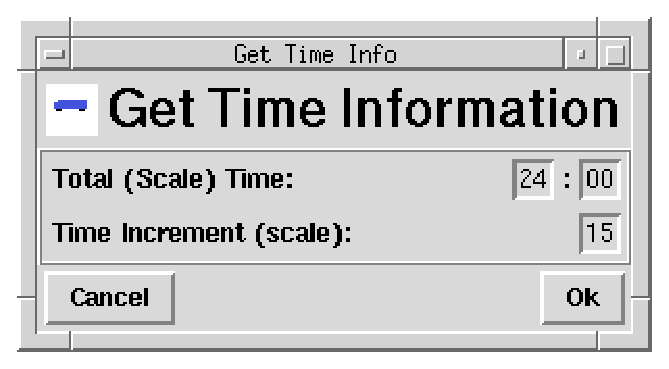
\epsfig{file=TimeTable/getTimeDialog.ps}\\
\caption{Get Time Information dialog box.}
\label{fig:getTimeDialog}
\end{centering}
\end{figure}

\section{Cab names and colors}

Next, your cab name and color information is collected by either
loading a cab file or with the ``Get Cab Info'' dialog box, as shown in
Figure~\ref{fig:getCabInfoDialog}.  The cab information is only needed
if you have an old-style switched DC cab control type of layout.  If you
are using a modern DCC type layout, you can cancel this dialog.  When
you add trains you will be asked for colors to draw the trains on the
chart, but these colors are only for ease of reference purposes.  After
loading the cabs you will have the option of saving the cab information
in a file.\footnote{See Appendix~\ref{chapt:Files} for information about
the format of this and other data files.}

\begin{figure}
\begin{centering}
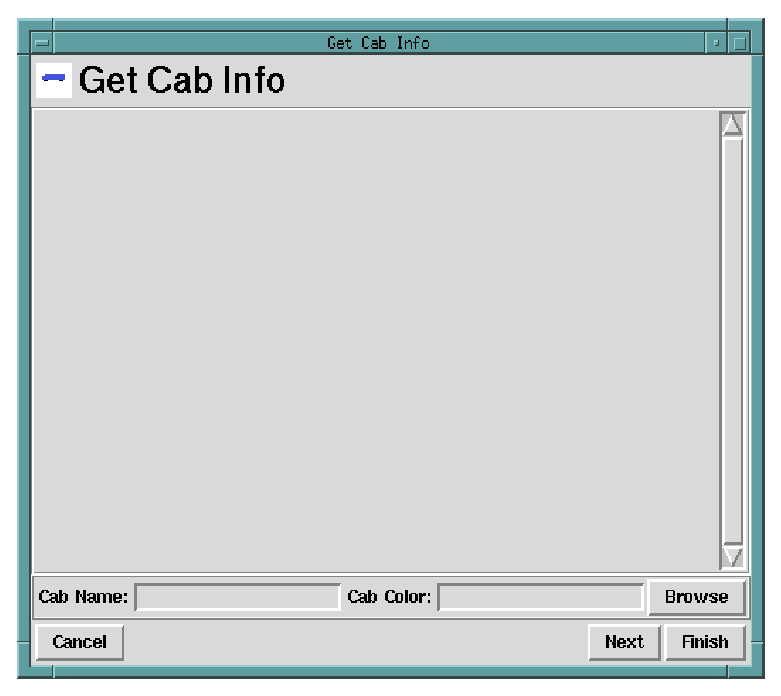
\epsfig{file=TimeTable/getCabInfoDialog.ps}\\
\caption{Get Cab Info dialog box.}
\label{fig:getCabInfoDialog}
\end{centering}
\end{figure}

\section{Getting Station List}
\label{sect:GettingStationList}

Next,  you will enter your stations and their distances down the line.
Either you can load a file with this information or you can use the
dialog box described below. 

The distances are presumed to be in $smiles$, which are scale miles
computed as shown in Equation~\ref{equ:smiles}.
\begin{equation}
Smiles = \frac{(DIS) (SF) (CR)}{5280}
\label{equ:smiles}
\end{equation}
where $(DIS)$ is the distance in real feet, $(SF)$ is your scale factor,
and $(CR)$ is your fast clock ratio.  It is possible to use
$skilometers$ instead.  These are computed as shown in
Equation~\ref{equ:skilometers}.  You will need to enter train speeds in
$skph$ instead of $smph$.
\begin{equation}
Skilometers = \frac{(DIS) (SF) (CR)}{1000}
\label{equ:skilometers}
\end{equation}
where $(DIS)$ is the distance in real meters, $(SF)$ is your scale
factor, and $(CR)$ is your fast clock ratio.

Once you have computed your station distances in $smiles$ (or
$skilometers$), you are ready to create your station list using the
``Get Station List'' dialog box, shown in
Figure~\ref{fig:getStationListDialog}.  The stations are the
vertical dimension of the chart, with the station names labeling
horizontal lines across the chart.  

\begin{figure}
\begin{centering}
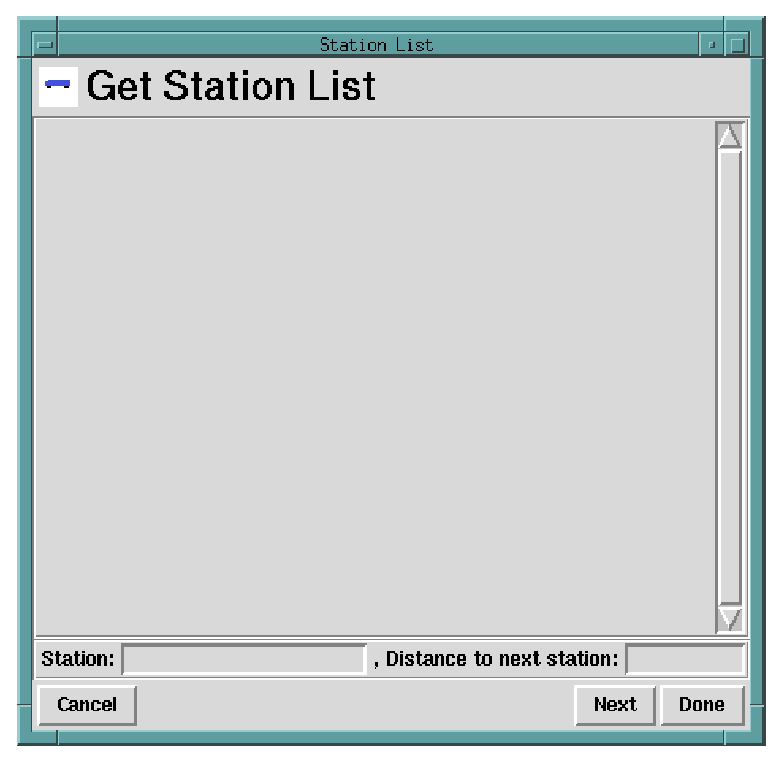
\epsfig{file=TimeTable/getStationListDialog.ps}\\
\caption{Get Station List dialog box.}
\label{fig:getStationListDialog}
\end{centering}
\end{figure}   

After getting the station list, a dialog box is presented to collect
your ``duplicate trackage''. The most common sort of duplicate trackage
occurs when you have an out and back type layout, which you are
graphing as if it is a either a continuous loop or an end-to-end
switching layout.  There is an example if Figure~8-4on page 86 of
\cite{Chubb77}. The ``Get Duplicate Trackage'' dialog box is shown in
Figure~\ref{fig:getDuplicateTrackageDialog}. Once you have entered your
stations you will have the option of saving them to a file.

\begin{figure}
\begin{centering}
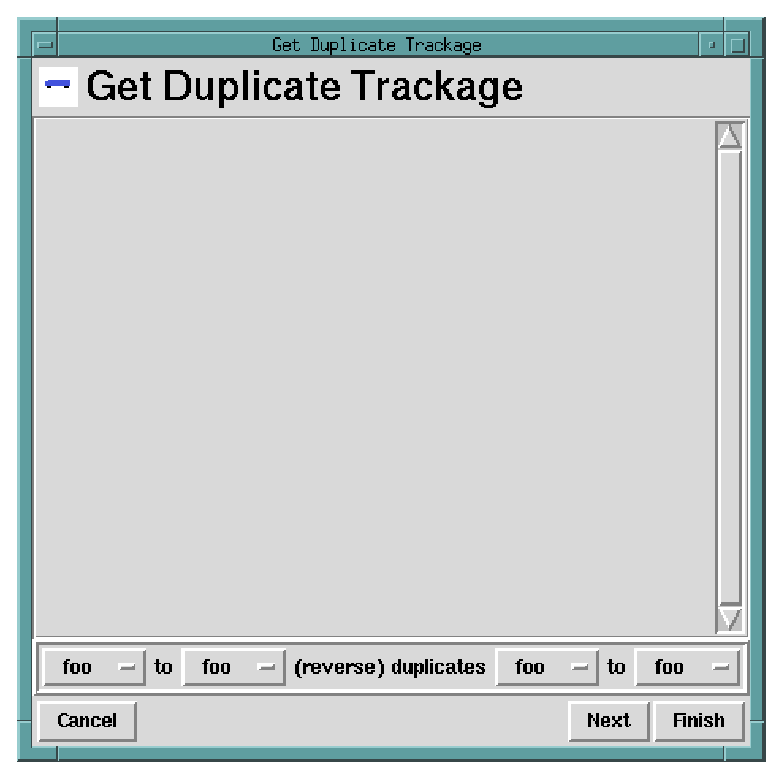
\epsfig{file=TimeTable/getDuplicateTrackageDialog.ps}\\
\caption{Get Duplicate Trackage dialog box.}
\label{fig:getDuplicateTrackageDialog}
\end{centering}
\end{figure}

Finally, you can load storage tracks from a file or use the ``Get
Storage Track'' dialog box to collect your storage tracks, as shown in
Figure~\ref{fig:getStorageTracksDialog}.  You will have the option of
saving your storage track information to a file once the information has
been entered.

\begin{figure}
\begin{centering}
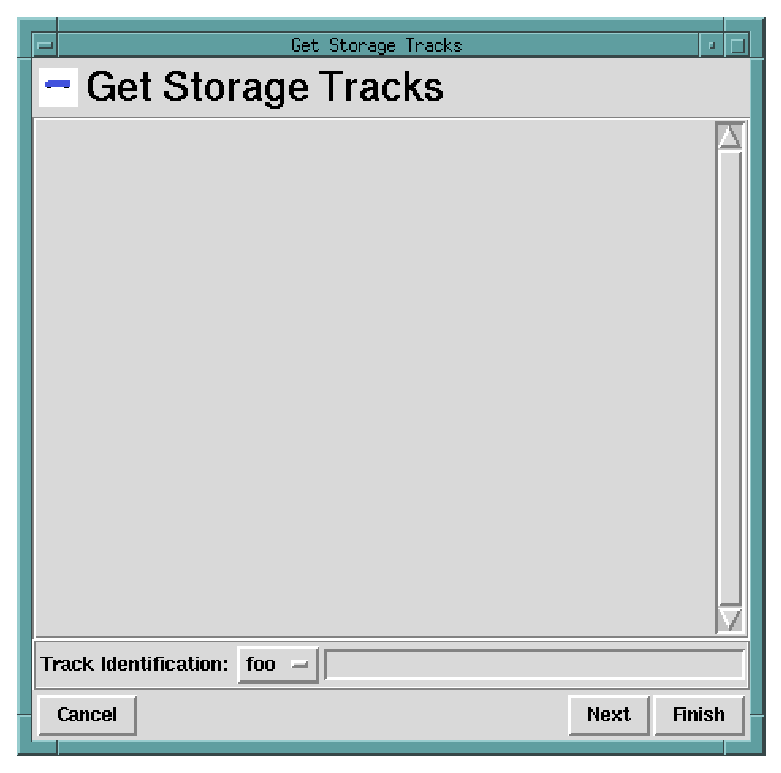
\epsfig{file=TimeTable/getStorageTracksDialog.ps}\\
\caption{Get Storage Track dialog box.}
\label{fig:getStorageTracksDialog}
\end{centering}
\end{figure}   

